Suprotstavljeno tradicionalnim operatorima križanja u genetskom programiranju koji ignoriraju semantiku samog programa, u \cite{crxSem} opisano je semantičko križanje. 
Ovo križanje razlikuje nekoliko inačica, od kojih je svaka primjenjiva na određenu vrstu problema. Semantičko križanje različito je definirano za situacije kada stablo jedinke predstavlja logičku ili realnu funkciju, ili ako je jedinka program.

Ukoliko jedinka predstavlja logičku funkciju, semantičko križanje definirano je kao:
 \begin{equation} 
\label{log}
 \large{ (T1 \land TR) \vee   (\overline{TR} \land T2) },
\end{equation}
gdje T1 i T2 predstavljaju roditelje koji sudjeluju u križanju, a TR predstavlja nasumično generirano stablo. Na slici \ref{semBool} prikazana je shema semantičkog križanja za logičke funckije.

 \begin{figure}[H]
	\centering
	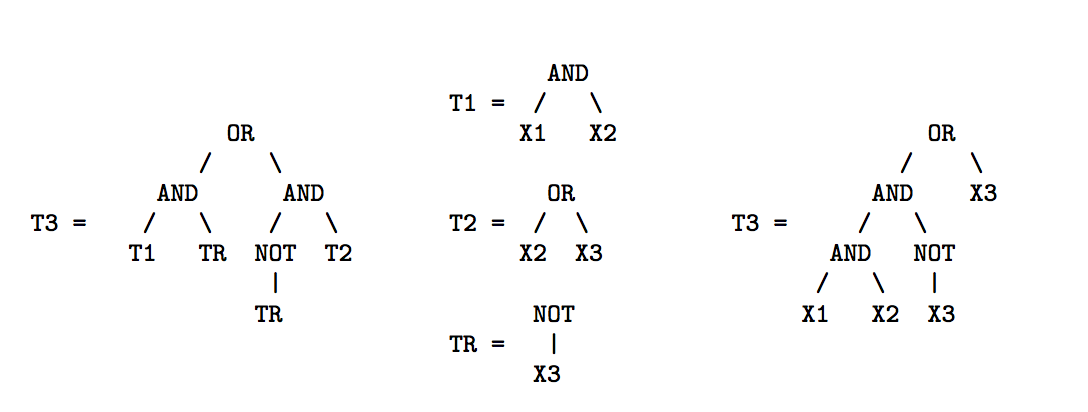
\includegraphics[scale=0.4]{./slike/semBool1.png}
	\caption{Lijevo: shema semantičkog križanja za logičke funkcije; sredina: roditelji i nasumično generirana jedinka; desno: rezultat križanja roditelja prikazanih u sredini (preuzeto iz \cite{crxSem})}
	\label{semBool}
\end{figure}
  
   
     Analogno ovome, za realne funkcije, odnosno, simboličku regresiju, semantičko križanje predstavljeno je sljedećim izrazom:
 \begin{equation} 
\label{log}
 \large{ (T1 \cdot TR) +   ((1-TR) \cdot T2) }.
\end{equation}
Za slučaj kada jedinka predstavlja program, semantičko križanje definira se kao:
 \begin{equation} 
\label{log}
 \large{ \textbf{IF}(CONDR) \textbf{THEN} (T1) \textbf{ELSE} (T2)},
\end{equation}
gdje je CONDR nasumično generiran program čiji je izlaz interpretiran kao logička vrijednost.

Iz ovoga je jasno vidljiv najveći nedostatak ovog operatora - prekomjeran rast novonastalih jedinki. Naime, prilikom svakog križanja stablo će se sigurno uvećati po dubini za barem jednu razinu. Ovo može postati znatan problem iz razloga što je rast vrlo brz, te se često nakon nekog vremena dogodi to da za novodobiveno stablo ne postoji prostor za pohranu. Radi ovoga, nakon svakog križanja, potrebno je pojednostavniti novonastalu jedinku. Ovo pojednostavljenje naravno mora osigurati da je funkcionalnost jedinke nakon pojednostavljenja ostala nepromijenjena.

Glavna prednost ovog semantičkog operatora je činjenica da je, za razliku od nekih drugih predloženih semantičkih operatora, primjenjiv na širok skup problema.

\subsection{Dosadašnji rezultati}

Eksperimenti u \cite{crxSem} provedeni su nad sve tri vrste problema za koje je ovaj operator definiran; logičke funkcije, simboličku regresiju i programe. Ovo istraživanje je usporedilo genetsko programiranje (\texit{GP}) sa semantičkim genetskim programiranjem (\textit{eng. semantic genetic programming - SGP}) i lokalnom pretragom (\textit{semantic stochastic hill climber - SSHC}). Također, napravljena je usporedba s algoritmom genetskog programiranja koje se vrti jednako dugo kao i SGP i SSHC za pojedini problem (\textit{GPt}). U nastavku su opisani dobiveni rezultati za pojedinu vrstu problema.

\subsubsection{Logičke funkcije}

Učinkovitost logičkog semantičkog operatora križanja provedena je na 5 različita problema, zajedno s nekoliko inačica za svaki problem. Problemi su redom: $n$ -komparator (6, 8 i 10), $n$ -multipleksor (6 i 11), $n$ -paritet (5, 6, 7, 8, 9 i 10), nasumično generirana funkcija $n$ varijabli (5, 6, 7, 8, 9, 10 i 11) i $n$-istinita funkcija \footnote{$n$-istinita funkcija je funkcija $n$ varijabli koja je za svaku kombinaciju varijabli istinita} (5, 6, 7 i 8). Dobrota je računata kao Hammingova udaljenost vrijednosti stvarne funkcije i dobivenog rješenja. Na slici \ref{semBoolTable} prikazana je tablica rezultata. 

Stupac \textit{Hits \%} predstavlja postotak uspješnosti nad skupom za učenje za najbolju jedinku u populaciji, za 30 pokretanja algoritma. Pri tome \textit{avg} predstavlja prosjek, a \textit{sd} standardnu devijaciju. U stupcu \textit{Length} prikazani su logaritmi po bazi 10 veličine dobivenih rješenja. Valja napomenuti da je nakon upotrebe semantičkog križanja primijenjena simplifikacija dobivenog rješenja, iz razloga što bi veličina rješenja eksponencijalno rasla u suprotnom. Vidljivo je kako SSHC i SGP konstantno pronalaze bolja rješenja od GP-a sa semantičkim križanjem, no GP proizvodi manje jedinke (čemu je glavni razlog pojednostavljenje izraza koje se u ostalim algoritmima ne obavlja - što umanjuje relevantnost ovog zaključka).  Vidljivo je kako GPt pokazuje bolje performanse od GP-a, no još uvijek se pokazuje lošijim od SGP-a i SSHC-a.

 \begin{figure}[H]
	\centering
	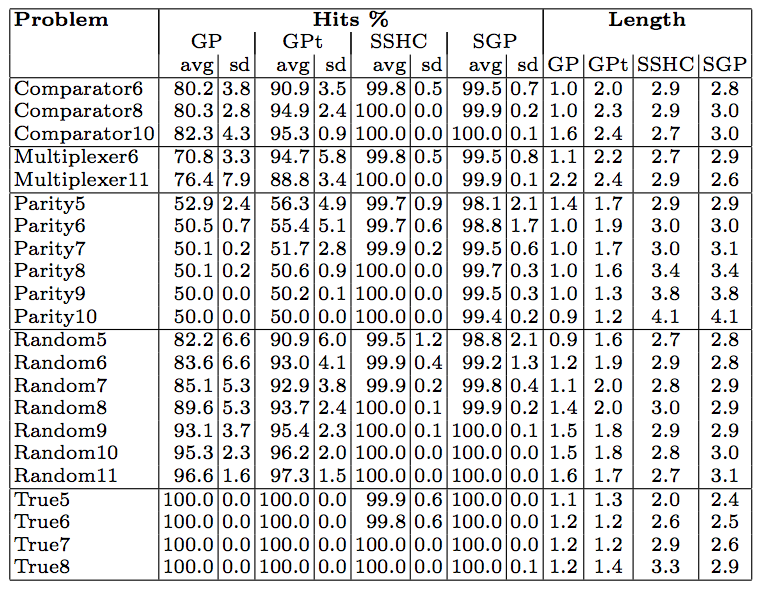
\includegraphics[scale=0.5]{./slike/semBoolTable.png}
	\caption{Usporedba učinkovitosti GP-a i GPt-a sa SGP-om i SSHC-om (preuzeto iz \cite{crxSem})}
	\label{semBoolTable}
\end{figure}

\subsubsection{Simbolička regresija}

Za ocjenu učinkovitosti ovog operatora na simboličkoj regresiji korišteni su različiti polinomi, od trećeg do desetog stupnja, s koeficijentima realnih vrijednosti iz intervala $[-1, 1]$. Funkcija dobrote računata je kao euklidska udaljenost stvarne funkcije i pronađenog rješenja. Na slici \ref{semSymbTable} prikazane su dobivene statistike provedenih eksperimenata.

 \begin{figure}[H]
	\centering
	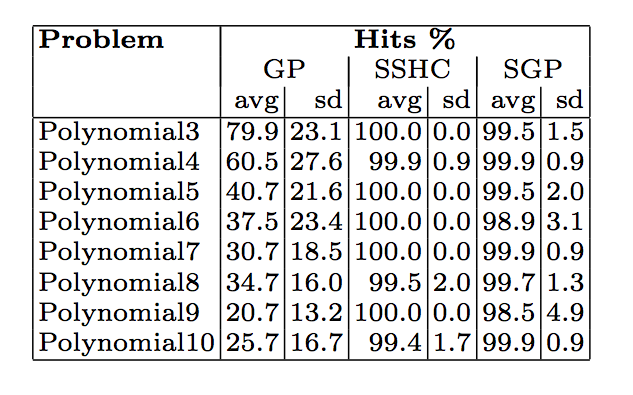
\includegraphics[scale=0.4]{./slike/semSymbTable.png}
	\caption{Usporedba učinkovitosti GP-a i GPt-a sa SGP-om i SSHC-om (preuzeto iz \cite{crxSem})}
	\label{semSymbTable}
\end{figure}

Vidljivo je kako je GP kao i u prethodnom slučaju, gori od SSHC-a i SGP-a, te da je standardna devijacija dosta veća nego kod ostalih.

\subsubsection{Programi}

Kako bi se pokazala učinkovitost semantičkog križanja nad programskim jedinkama, korišten je problem klasifikacije u jednu klasu na osnovu dvije značajke ($(n_c, n_v) \to n_ {cl}$). Na slici \ref{semProg} prikazani su rezultati eksperimenata. Ovdje je ponovno pokazana inferiornost GP-a naprema SSHC-u i SGP-u.

 \begin{figure}[H]
	\centering
	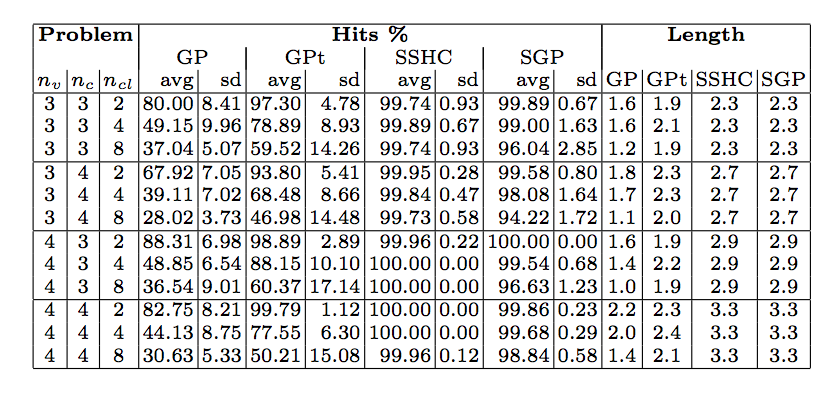
\includegraphics[scale=0.5]{./slike/semProg.png}
	\caption{Usporedba učinkovitosti GP-a i GPt-a sa SGP-om i SSHC-om(preuzeto iz \cite{crxSem})}
	\label{semProg}
\end{figure}

Unatoč prikazanim rezultatima, autori \cite{crxSem} tvrde da ovaj operator križanja djeluje bolje od uobičajenih operatora u genetskom programiranju. No, za to nisu priložili nikakav dokaz. U sklopu ovog rada implementirano je ovakvo križanje, te će u kasnijim poglavljima biti prikazana usporedba učinkovitosti ovog operatora s onim operatorima koji su opisani u prethodnim poglavljima.